
\chapter{Learning To Compose Grounded Spatial Relations}
\chaptersource{Mehdi Ghanimifard and Simon Dobnik.}{Learning to Compose Spatial Relations with Grounded Neural Language Models.}{In Proceedings of 12th International Conference on Computational Semantics (IWCS)-Long papers. 2017.}

\paragraph{Abstract}
Language is compositional: we can generate and interpret novel sentences by
having a notion of meaning of their individual parts. Spatial descriptions are
grounded in perceptional representations but their meaning is also defined by
what neighbouring words they co-occur with.
In this paper we examine how language models conditioned on perceptual features
can capture the semantics of composed phrases as well as of individual words. We
generate a synthetic dataset of spatial descriptions referring to perceptual
scenes and examine how grounded language models built with deep neural
networks can account for compositionality of descriptions -- by evaluating how
the learned language models can deal with novel grounded composed descriptions and novel
grounded decomposed descriptions, constituents previously not seen in isolation.

\section{Introduction}
Representing and reasoning with linguistic meaning is a central task in
computational linguistics. Here two kinds of meaning representations are used:
(i) \emph{probabilistic language models} and
(ii) \emph{meaning representations grounded} in other, typically perceptual
information. Recently, there have been several approaches in deep learning that
deal with both, either independently or together.

The main goal of \emph{probabilistic language models} is to estimate a
probability distribution of sequences of words based on observable samples
from language production, typically by estimating conditional
probabilities of words with a categorical distribution. This gives language
models means for representing words as sequences with a measure of likelihood
for each sequence. Neural language models perform this objective by
parametrising a probability density function with parametric representations
of words and functions which compose words into phrases
\cite{bengio2003neural,mnih2007three,mikolov2010recurrent}. The gradient based
learning in neural networks turns the modelling problem into an optimisation problem,
minimising the error or distance between a model prediction and an observable
data over a list of parameters:
\begin{enumerate}[topsep=0em,itemsep=0em,partopsep=0em,parsep=0em]
\item[1.] parameters representing words with feature vectors known as
\textit{word embeddings};
\item[2.] parameters of functions composing word features into a
structure; %
\item[3.] parameters of projections from final composed representations to
categorical probabilities which in sequential models are the next word predictions.
\end{enumerate}

There have been many attempts to show that the learned word embeddings in vector
spaces are good representations of meaning. Basing the argument on
the distributional hypothesis, if a probabilistic model of words is conditioned on
their context words (i.e. skip-grams or bag-of-words), the word embeddings must
encode semantic information by having learned distances in vector spaces which
correspond to semantic similarity scores obtained through relatedness tests performed by native speakers. These representations
were extended to word compositions by considering different compositional functions as vector manipulations
\cite{mitchell2010composition,coecke2010mathematical,baroni2014frege}.
Our notion of composition in a language model is broader
than this: it involves (1) distributional models of words estimated from word
sequences as well as (2) their grounding into representations of physical space.
This extends the Montague's notion of compositionality. Lexical
representations and their compositions are not dependent on meaning postulates and lexicalised constraints
but rather perceptual evidence which is (probabilistically) associated with them.

\cite{harnad1990symbol,roy2005semiotic} define language grounding as a process
of relating words with an agent's perception. The ambiguity and
vagueness of grounded meanings as well as of syntactic structures suggest that the
connection between language and perception is gradient and therefore
probabilistic. The main approaches to probabilistic models of grounded language
are probabilistic learning of grounded language and grammar
\cite{roy2005towards,matuszek2012joint}, classifiers \cite{Dobnik:2009dz}, and feature representations in perceptual space such as colour \cite{mcmahan2015bayesian}. Our proposal is in line with all three approaches. 

A \emph{grounded language model} is a language model conditioned by 
perceptual representations that it refers to. Ideally, the model should capture
how each constituent in the composed phrase relates to some perceptual
representations. For example, in an image captioning task, a grounded language
model estimates a conditional probability of a word sequence
$w_{1:T}$ given some image feature $c$ that the words refers to. A
general way to model word sequences is to use the chain rule as
follows. The model can generate phrases and sentences step-by-step by predicting
the next word in a sequence:
\begin{equation}\label{iwcs2017:eq:lm}
 Pr(w_{1:T} | c) = \prod_{t=1}^{T}{Pr(w_{t} |w_{1:t}, c)}
\end{equation}
The parametrisation of vision and language is often done by
combining word-embeddings with multimodal embeddings
\cite{kiros2014unifying,socher2014grounded}.
In the state of the art models for image captioning with encoder-decoder
architecture, the encoder module is trained under the assumption
that grounded words only denote features in subareas of an image, e.g bounding
boxes \cite{karpathy2015deep} and pixel-wise mapping with attention models
\cite{xu2015show,lu2017knowing}.
Another example of a visually grounded language model is a model that is used to demonstrate
the compositionality of colour descriptions in \cite{monroe2016learning} where 
linguistic descriptions are associated with areas of the colour space. Similar to \cite{mcmahan2015bayesian},
each observed instance is a colour term paired with a colour code but instead
of considering each description as a lexical entry, phrases are captured by
a grounded language model as in Equation~\ref{iwcs2017:eq:lm}. The
qualitative human evaluation of how newly composed colour words by this model refer
to the colour space suggest that language models can capture compositionality
through gradient learning used with neural networks.

In this paper, we follow up and extend the work of \cite{monroe2016learning}.
We focus on recurrent neural language models of sequences of words conditioned by encoded locations
that these words refer to in visual scenes. Hence, we are interested in
grounded semantic composition that is not only captured by probabilistic models of words
given their context words, but also by models of their relatedness to
perceptual representations. An important and novel question we investigate is
\emph{what these models are learning}: to what degree the representations of
meaning (both collocational from vector spaces and grounded in perception) are
interpretable and therefore \emph{compositional} in the sense of
\cite{Montague1974}. We focus on one domain of grounded meaning: spatial
descriptions of various length and their grounding in spatial templates of
\cite{logan1996computational}. In particular we try to answer the following questions:
\textit{(1)} To what extent are the language models that have been learned grounded in
spatial representations?
\textit{(2)} Is it possible to generate new, previously unseen grounded composed
spatial descriptions from observing their words only in other grounded composed
phrases?

This paper is organised as follows. In Section~\ref{iwcs2017:sec:dataset} we describe the
creation of an artificial dataset of composed spatial templates and the
associated descriptions based on the experimental work of
\cite{logan1996computational}. In Section~\ref{iwcs2017:sec:anns} we describe our neural
network model which we use for training our grounded language model.
Section~\ref{iwcs2017:sec:evaluation} describes an evaluation of the learned
representations compared to the original representations the system was learning
from. Finally, Section~\ref{iwcs2017:sec:conclusions} points to conclusions and further
work. The code and results are available at
\url{https://github.com/GU-CLASP/spatial-composition}.

\section{The dataset}\label{iwcs2017:sec:dataset}
In order to train a grounded language model we require samples of language use
paired with locations they are referring to. Considering the rationality of
speakers and their observers \cite{Grice:1975aa}, the frequency of each
co-occurring utterance--location corresponds to the appropriateness of such
utterance as a description of that location. One complication of judging
the appropriateness of spatial terms this way is that they are not only depended on the
location they describe but also on other properties of the situation such as the
agreed frame of reference, object shape, and the function of the landmark and
the target objects involved, etc. \cite{herskovits1986language,Dobnik:2016ad}. However, these properties will not be
considered in the present study.

\cite{logan1996computational} performed several psychological experiments related to the geometric apprehension of
spatial relations. For example, %
they collected
acceptability ratings (1--9) for a set of spatial relations per different
locations of the target object in a $7 \times 7$ grid relative to the landmark object in the centre ($3,3$). The acceptability scores were
collected from 32 informants through random presentation and then averaged per location. The matrix of average acceptability scores per description is called a \textit{spatial template} and represents the appropriateness
of each location in the process of interpreting that spatial relation
\cite{logan1996computational}.
They collect spatial templates for the following spatial relations:
\textit{right\_of}, \textit{left\_of},
\textit{below}, \textit{under}, \textit{over}, \textit{above},
\textit{near\_to}, \textit{next\_to}, \textit{far\_from}, and \textit{away\_from} which we also apply in our work. Furthermore, in order to be able to explore the limits of the language models for learning
compositions, we extend this vocabulary with a few additional words.
We describe how we used them to synthesise the composed spatial templates for our training data in the following section.

\subsection{Spatial templates as probabilities}

As stated earlier, the spatial templates of \cite{logan1996computational} give
us the average acceptability scores on the scale 1--9 for each of $7 \times 7 - 1$
locations. In the process of grounding a description ($w_{1:T} = w_1 w_2 \ldots
w_T$), a vector of scores representing its spatial template is used to rank
the description's acceptability across all possible locations:
\begin{equation}
T_{w_{1:T}} = \{Score(w_{1:T}, l)\}_{l \in L}
\end{equation}
Our goal is to find such representation for any composed phrase $w_{1:T}$.
We introduce the following assumption to convert the acceptability scores to probabilities. The
acceptability scores are an indicator of a degree of belief \cite{ramsey1931truth}
that a rational speaker would use a particular description ($w_{1:T}$) to
describe the landmark object at a certain location ($c \in L$). We therefore expect:
\begin{equation}\label{iwcs2017:eq:rational}
  Score(w_{1:T}, c) \propto Pr(w_{1:T}, c)
\end{equation}
\noindent where the $Pr(w_{1:T}, c)$ is the probability of observing a co-occurrence of a
phrase $w_{1:T}$ and a location $c$. In order to be able to compare spatial
templates generated by the learned neural language models and the original acceptability scores
which were used to generate the training data, we assume that all locations are
equally accessible, then:
\begin{equation}\begin{array}{l}
   Pr(w_{1:T}, c) = Pr(w_{1:T} | c) Pr(c) \\
   \implies Score_(w_{1:T}, c) \propto Pr(w_{1:T} | c) \\
\end{array}
\end{equation}
We compare the generated probability scores by our neural language model, a vector of
probabilities over all locations, for a particular description with its expected spatial
template. We use a correlation coefficient to quantify the difference between
a predicted and the ``real'' spatial template. A
spatial template gives us information about the applicability of each location.
When choosing a location given a description we would consider the ranking of
locations by their applicability score. Hence, since we are not interested in
the actual scores but their ranking, Spearman's rank correlation coefficient is
a suitable measure for comparing spatial templates.
\begin{equation}\label{iwcs2017:eq:sptemp}\begin{array}{r c l}
T_{w_{1:T}} &=& \{Score_{w_{1:T}, l}\}_{l \in L} \\
\hat{T}_{w_{1:T}} &=& \{Pr(w_{1:T} | c) \}_{l \in L} \\
\rho(T_{w_{1:T}}, \hat{T}_{w_{1:T}}) & &\textrm{Spearman's rank correlation
coefficient}
\end{array}
\end{equation}
\subsection{Synthesised data}\label{iwcs2017:sec:synth}

Considering the assumptions from the previous section, using a simple min-max normalisation, the
list of scores in a spatial template can be translated to a Bernoulli
probability of events:
\begin{equation}
Pr(w_{0:T}, c) \approx s_{w_{1:T}, c} = \frac{Score(w_{1:T}, c) - 1}{9 - 1}
\end{equation}
\noindent Using these probabilities, we synthesise instance events of 
locations and descriptions that make our training dataset using the same method as \cite{coventry2004spatial}. Having normalised acceptability ratings as probabilities, 
we can generate samples with a frequency corresponding to these probabilities.
\begin{equation}
freq(w_{0:T}, c) = n \times Pr(w_{0:T}, c) %
\end{equation}
\noindent For example, by choosing $n=5$, for a location with normalised scores 0.58 for
$right\_of$, 0.15 for $left\_of$ and $0.91$ for $next\_to$,
we generate 2, 0, 4 instances for each respective description.

\cite{logan1996computational} present acceptability scores for spatial
descriptions obtained experimentally only for single-word spatial descriptions
such as $left$ and $above$. However, in our task we need their composed
representations.
We take the assumption that all spatial templates compose with some known
function. For example for two spatial descriptions conjoined with an
intersective $and$ ``\{spatial\_term1\} and \{spatial\_term2\}'',
\cite{Gapp:1994:CompositeRelations} discusses (but not experimentally evaluates) five compositional functions for grounding spatial templates. More recently, \cite{Dobnik:2017ac} show that taking a
\emph{geometric mean} over acceptability scores per location give highly
correlated compositions with spatial templates of composed descriptions obtained
experimentally. Another study on representing binary beliefs with beta
distributions \cite{josang2005multiplication}, shows that the product of scores 
has the best approximation for conjoined opinions. We also take this as our
compositional function to generate spatial templates for composite descriptions
as in Figure~\ref{iwcs2017:fig:composition}, here further defined as:
\begin{equation}\begin{array}{r c l}
g_\land &:& (v_i, v_j) \to[v_i,``\mathrm{and}",v_j] \\
\hat{s}_{g_\land(v_i,v_j),c} &=& s_{v_i, c} \times s_{v_j, c}
\end{array}
\end{equation}
\noindent Where $g_\land$ is a grammar rule for conjoined composition. Similarly, following \cite{josang2005multiplication}, logical OR-composition can be defined with
co-multiplication:
\begin{equation}\begin{array}{r c l}
g_\lor &:& (v_i, v_j) \to [``either",v_i,``\mathrm{or}",v_j] \\
\hat{s}_{g_\lor(v_i,v_j),c} &=& s_{v_i, c} + s_{v_j, c} - s_{v_i, c} \times s_{v_j, c}
\end{array}
\end{equation}
\noindent For negation ``not \{spatial\_term\}'' we take a complement of the acceptability
scores as shown in Figure~\ref{iwcs2017:fig:composition}.
\begin{equation}\begin{array}{r c l}
g_\neg &:& v \to [``\mathrm{not}",v] \\
\hat{s}_{g_\neg(v),c} &=& 1 - s_{v, c}
\end{array}
\end{equation}
\begin{figure}[hbt]
\centering
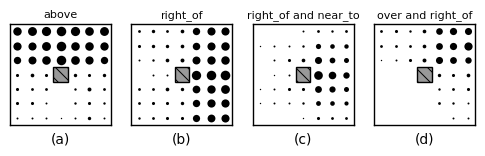
\includegraphics[scale=0.85]{studies/iwcs2017/images/compositions_abcd.png}
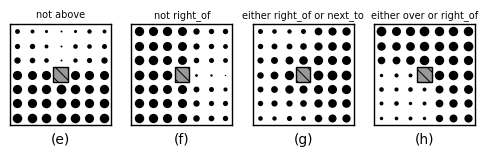
\includegraphics[scale=0.85]{studies/iwcs2017/images/compositions_efgh.png}
\caption{\label{iwcs2017:fig:composition}
Spatial templates in a $7 \times 7$ grid:
(a) and (b) are spatial templates for ``above'' and ``right'' from
\cite{logan1996computational} collected from human judgements. (c-h) are
their synthetic compositions. (c) and (d) are
intersective-AND compositions of two spatial templates using point-wise 
multiplication. (e) and (f) represent the negation of (a) and (b) using a
complement operation. (g) and (h) are logical-OR compositions of two spatial templates
using a point-wise co-multiplication.}
\end{figure}
The resulting compositions are shown in Figure~\ref{iwcs2017:fig:composition}. One might object to the usage of such synthetic data. It is important to note
that the prime goal of this work is not to learn grounded models of spatial
language that would best approximate human intuitions but to test to what degree
grounded neural language models are capable of capturing grounded
compositionality expressed as compositional functions of various complexities which have been confirmed in the previous literature to work well. Hence, we are interested in
testing to what extent new machine learning models are capable of learning these functions.

We create two datasets. In the first dataset all descriptions are grounded in
spatial templates as described above. In the second dataset additional
words were added which we assume have no grounding in perception to test if the neural
language model is able to distinguish them from the words sensitive to grounding. For
example: ``\{the object $|$ it $|$ the ball\} is \{spatial\_phrase\} \{the
object $|$ it $|$ the box\}''. The following additional grammar rules
were applied during the generation of the second dataset:
\begin{equation}\label{iwcs2017:eq:grammar-rules}
\begin{array}{r c l}
g_1 &:& (v*) \to [v*] \\
g_2 &:& (v*) \to [``it", ``is", v*] \\
g_3 &:& (v*) \to [``it", ``is", v*, ``the'', ``box''] \\
g_4 &:& (v*) \to [``the", ``ball", ``is", v*, ``the'', ``box''] \\
g_5 &:& (v*) \to [``the", ``object", ``is", v*, ``the'', ``box''] \\
\end{array}
\end{equation}%
\begin{algorithm}
\caption{Synthetic generator}\label{iwcs2017:alg:generator}
\begin{algorithmic}[1]
\State $\textit{n} = 5$
\State $g_{compositional} = \{g_1, g_\neg, g_\land, g_\lor\}$
\State $g_{textual} = \{g_1, g_2, g_3, g_4, g_5\}$
\Procedure{SyntheticGenerator}{$v*, c, g$}
\State $freq \gets n \times \hat{s}_{g(v*), c}$
\For{$1\ \mathbf{to}\ freq$}
\State $syntax \gets \mathrm{choose\_random}(g_{textual})$
\State $text \gets syntax(g(v*))$
\State $\mathbf{Generate}(text, c)$
\EndFor
\EndProcedure
\end{algorithmic}
\end{algorithm}
In the generated descriptions, words such as \textit{and, not, the, box, ball,
it, object,} and \textit{is} are not grounded in locations individually but the phrases they occur in refer to
locations on the map.

\section{Neural network architecture}\label{iwcs2017:sec:anns}

We use the Recurrent Neural Network (RNN) architecture
for a language model \cite{graves2013generating} with Long-Short Term Memory
(LSTM) \cite{hochreiter1997long} and a decoder architecture from
\cite{cho2014learning} which concatenates word-embeddings of each input word with an encoded location:
\begin{equation}
\begin{array}{r c l}
  \mathbf{y}_t &=& Pr(w_t| w_{1:t-1},c)  \\
  \mathbf{h}_t &=& f_{\theta}(\mathbf{e}_{w_{t-1}};\mathbf{c}, \mathbf{h}_{t-1}) \\
  \mathbf{\hat{y}}_t &=& \mathrm{softmax}(\mathbf{W} \mathbf{h}_t+\mathbf{b})
\end{array}
\end{equation}
\noindent where $\mathbf{\hat{y}}_t$ is the expected categorical probability
at time $t$, $f$ is a recurrent cell with parameters $\theta$,
$\mathbf{e}_w$ is an embedding vector for a word $w$, and $\mathbf{c}$ is an
encoded location as a one-hot vector as shown in Figure~\ref{iwcs2017:fig:rnnmodel}.
\begin{figure}[h]
\centering
\begin{tabular}{p{0.25\textwidth} p{0.75\textwidth}}
\vspace{0pt} 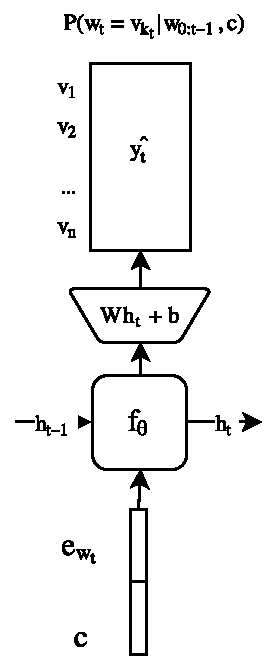
\includegraphics[scale=0.4]{studies/iwcs2017/RNN_Model_Diagram_partial.pdf} &
\vspace{0pt} 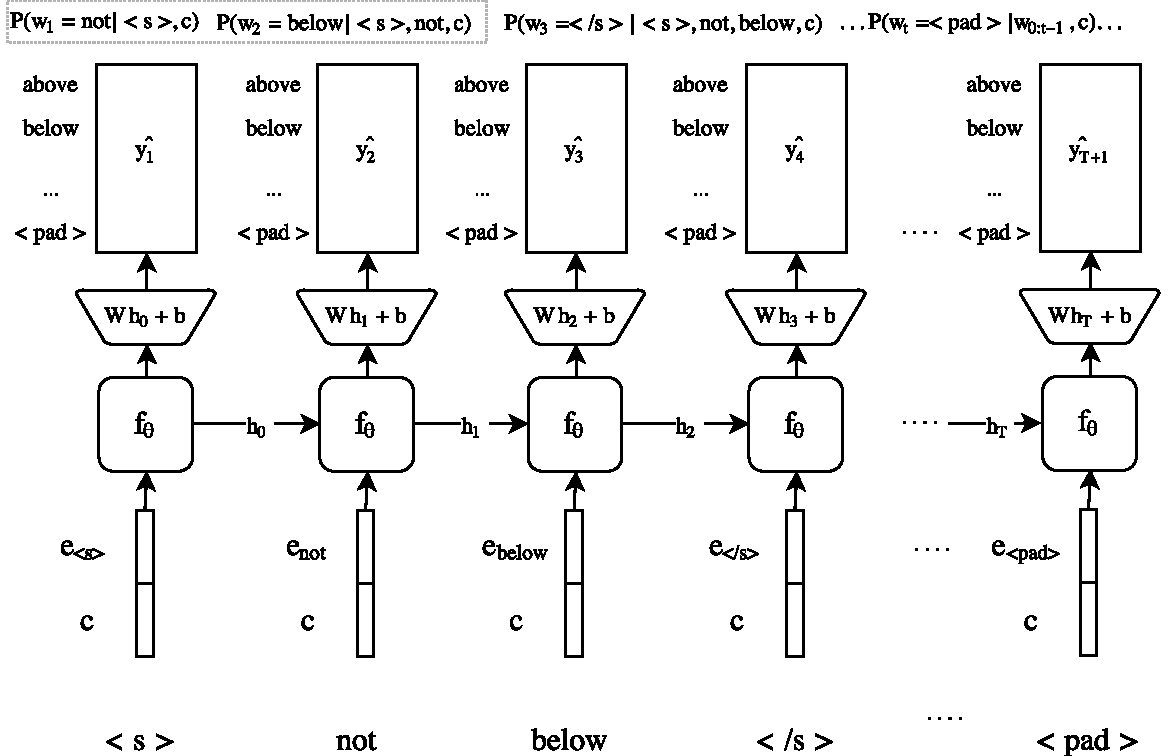
\includegraphics[scale=0.4]
{studies/iwcs2017/RNN_Model_Diagram.pdf}
\end{tabular}\vspace{0.5em}
\caption{\label{iwcs2017:fig:rnnmodel} The diagram on the left illustrates the
architecture of the model at word/time-step $t$ using a vocabulary size $n$. On the
right, there is an unfolded example how a phrase like ``not below'' is paired with a
location $c$ as in $(w_{1:T}, c)$ and fed as input to the LSTM decoder.
In this setup, similar to \cite{graves2013generating}, we train the model to
predict the next word in a sequence and the chain of output probabilities is taken to estimate
the final probability. The sequence can be cut before reaching the end tag
$</s>$. }
\end{figure}

The training set in a batch are pairs of word sequences and their corresponding
location codes: $\{({w^{(i)}}_{1:T}, c^{(i)})\}_{i \in D}$ where $D$ is our
training dataset. The loss function used is the cross entropy distance between
predicted distribution and targeted distribution or \emph{log-loss}. The
observed true output $\mathbf{y}^{(i)}_t$ is represented with one-hot encodings.
The training process can be summarised as follows:
\begin{equation}\label{iwcs2017:eq:log-loss}
\begin{array}{r c l}
  \mathbf{y}^{(i)}_t &=& \delta_{w^{(i)}_t} \\
  L^{(i)}(\Theta) &=& -\sum_{t=1}^{T+1}{\mathbf{y^\mathrm{T}}^{(i)}_t  \textrm{log}(\mathbf{\hat{y}}^{(i)}_t)} \\
  & = & -\sum_{t=1}^{T+1}{\textrm{log}(\mathbf{\hat{y}}^{(i)}_t(w^{(i)}_t))}
\end{array}
\end{equation}
\noindent We train the network parameters with \emph{Adam stochastic gradient descent}
\cite{kingma2014adam} with batch normalisation implemented as an optimiser in
Keras \cite{chollet2015keras}. On each mini-batch update as ($\Theta_{b} \leftarrow
\Theta_{b-1} + AdamSGD(\nabla_{\Theta} \mathcal{L})$) the following parameters of the model ($\Theta$) 
are updated:
\begin{equation}
\begin{array}{l l}
  \{\mathbf{e}_w\}_{w \in V}\ & \textrm{Embedding vectors for all words} \\
  \theta & \textrm{Parameters of the RNN cell, composed feature vectors}\\
  \mathbf{W}, \mathbf{b} & \textrm{Parameters of the final dense layer} \\
\end{array}
\end{equation}

\subsection{Implementation}

We implemented our model in Keras \cite{chollet2015keras} with TensorFlow
\cite{tensorflow2015-whitepaper} as a back-end. All parameters were initialised
randomly with Keras recommendations. In the current implementation, the size of
the $\mathbf{h}_t$, the hidden unit of LSTM, is 15, and the parameters of the
RNN cell have a dropout of 0.1. The dropout on embeddings is set to 0.3.

We left-padded descriptions $w_{1:T'}$ with a starting token $w_0 = <s>$ and
right-padded them with a finishing token $w_{T'+1}=</s>$ while the rest was
padded with $<pad>$ up to the maximum description length of $T+1$ as illustrated in
Figure ~\ref{iwcs2017:fig:rnnmodel}. The final $y_{T+1}$ can be either $<pad>$ or $</s>$.
The length of the RNN chain has to be of the fixed size $T+1$, the length of the
longest possible sentence, in order to be used with Keras and its implementation
on graphic cards.

During each experiment, we trained the model until it reached an over-fitting
point with equal training and validation loss.

\subsection{From the outputs of the RNN to probabilities of composed descriptions}

The decoder architecture of RNNs is normally used as a generator which produces
sequences of words or characters from an encoded sequence, e.g.
\cite{cho2014learning,graves2013generating}. This can be achieved by applying 
Equation~\ref{iwcs2017:eq:lm}. The decoder predicts the most likely next word in a chain of
softmax productions $\hat{\mathbf{y}}_t$.  The unfolded RNN in Figure~\ref{iwcs2017:fig:rnnmodel} shows how for a sequence of words as input vectors,
$\hat{\mathbf{y}}_t$ are predicted which represent categorical probabilities for all
possible following words at a time step $t$. For a given sequence, $w_{1:T} =
v_{k_1:k_t}$, we estimate the probabilities using Equation~\ref{iwcs2017:eq:lm} 
as follows:
\begin{equation}\begin{array}{r c l}
	Pr(w_t=v_{k_t}|w_{1:t-1}=v_{k_1:k_t}, c) &=& \hat{\mathbf{y}}_t(v_{k_t}) \\
Pr(w_{1:T}=v_{k_1:k_T} | c) &=& \prod_{t=1}^{T}{\hat{\mathbf{y}}_t(v_{k_t})} \\
\end{array}
\end{equation}
\noindent The estimated probability is then used to generate spatial templates as in
Equation~\ref{iwcs2017:eq:sptemp}. The probabilities over all possible
locations on the map $L$ for a given composition of words can be aggregated as follows:
\begin{equation}
\hat{T}_{v_{k_1:k_{T'}}} = \{Pr(w_{1:{T'}}=v_{k_1:k_{T'}} | c)\}_{c \in L}
\end{equation}

\section{Evaluation}\label{iwcs2017:sec:evaluation}

We evaluate the learning of composed grounded phrases by examining to what degree the
spatial templates produced by the learned model correspond to the original
spatial templates that were used in generating the training data, how successful is the learning with
different kinds of compositions, and what is the effect of adding distractor words. We ran two
experiments, (1) on a simple synthetic dataset containing short phrases where
all words are grounded in locations, and (2) on a synthetic dataset
generated with five additional grammar rules from Equation~\ref{iwcs2017:eq:grammar-rules}, introducing
words without spatial grounding or distractor words. We test the learning of compositional phrases by training a language model on phrases produced by individual composition types as well as all composition types in both synthetic datasets. A comparison of the
predicted spatial templates with the original spatial templates with Spearman's rank
correlation coefficient (Equation~\ref{iwcs2017:eq:sptemp}) in Table~\ref{iwcs2017:tab:exp0} shows that there is high
correlation between them. We
report the average Spearman's $\rho$ and their median p-values for statistical significance.

\begin{table}[htbp]
\centering
\small
\begin{tabular}{lrrr}
\hline
 &    Simple phrases &  With distractors & Untrained \\
\hline
AND-phrases         &  0.87 &      0.85& -0.00\\
NEG-phrases         &  0.72 &      0.82&  0.03\\
OR-phrases          &  0.79 &      0.80& -0.03\\
SINGLE-word         &  0.92 &      0.91& -0.05\\
All previous               &  0.83 &      0.83& -0.01\\
All previous + distractors &  NaN  &  0.84& -0.03\\
\hline
\end{tabular}\vspace{0.5em}
\caption{\label{iwcs2017:tab:exp0} For each type of compositional phrases we calculate
the average Spearman's rank correlation coefficient ($\rho$)
between the predicted spatial templates and
the templates used to generate the training data. The median p-value of $\rho$ of all trained models
is $<0.001$. The column \emph{Untrained} indicates the performance of the model
with a random initialisation of weights.} %
\end{table}

For both Experiment 1 and 2 we created two variations:
(1) learning of novel grounded compositions, where different
proportions of AND-phrases and OR-phrases are omitted from the dataset and
therefore hidden from the learner;
(2) learning of novel single words from grounded compositions, where
proportions of single-word instances are omitted from the dataset and their
representations can only be learned from their occurrence in
composed phrases with other words.

In all experiments we hold out 10\%  of the dataset for validation. In
Experiment 1 we iterated the training over 64 epochs using a batch size 8. In
Experiment 2, using a batch size 256, we stopped learning iterations before
1024 epochs if the validation loss became equal to the training loss.

\subsection{Experiment 1: Learning composition of short phrases}

In this experiment the training data is generated for single spatial words,
AND-compositions, OR-compositions, and negated phrases without additional distractor words save ``and'', ``either'', ``or'', and ``not''.

\subsubsection{Learning of novel grounded compositions}

The training data contains synthesised samples of all single words
and their negations. However, different proportions of AND-phrases and
OR-phrases are removed from the training set to test if the model can learn unseen
composed phrases. Table~\ref{iwcs2017:tab:exp1} shows the average of Spearman's
$\rho$ correlation coefficient for different portions of held-out phrases.
Figure~\ref{iwcs2017:fig:exp1:sample2} illustrates some predicted novel grounded
compositions where 50\% of complex phrases were held out. The $\rho$
scores lower than 0.6 may not be trustworthy, e.g. ``above and left\_of'' with
$\rho=0.5$ in Figure ~\ref{iwcs2017:fig:exp1:sample2}.

\begin{table}[htbp]
	\centering
	\small
	\begin{tabular}{m{5.7em}c@{\hspace{0.7em}}c@{\hspace{0.7em}}c@{\hspace{0.7em}}c@{\hspace{0.7em}}c@{\hspace{0.7em}}c@{\hspace{0.7em}}c@{\hspace{0.7em}}c@{\hspace{0.7em}}c@{\hspace{0.7em}}c@{\hspace{0.7em}}}	
	\hline
	Proportions of 90 combinations &   10\% &   20\% &   30\% &   40\% &   50\% &   60\% &   70\% &   80\% &   90\% &   100\% \\
	\hline
	AND-phrases & 0.84 &  0.8 & 0.78 & 0.76 & 0.71 & 0.67 & 0.64 & 0.53 & 0.45 &  0.29 \\
	OR-phrases  & 0.74 & 0.73 & 0.69 & 0.67 & 0.56 & 0.57 & 0.54 & 0.38 & 0.23 & -0.23 \\
	\hline
	\end{tabular}\vspace{0.5em}
	\caption{\label{iwcs2017:tab:exp1}
	Spearman's $\rho$ for held-out proportions of phrases. up to 80\% have a median
	p-value $<0.001$ and p-value $>0.05$ for higher proportions.}
\end{table}
\begin{figure}[htbp]
\centering
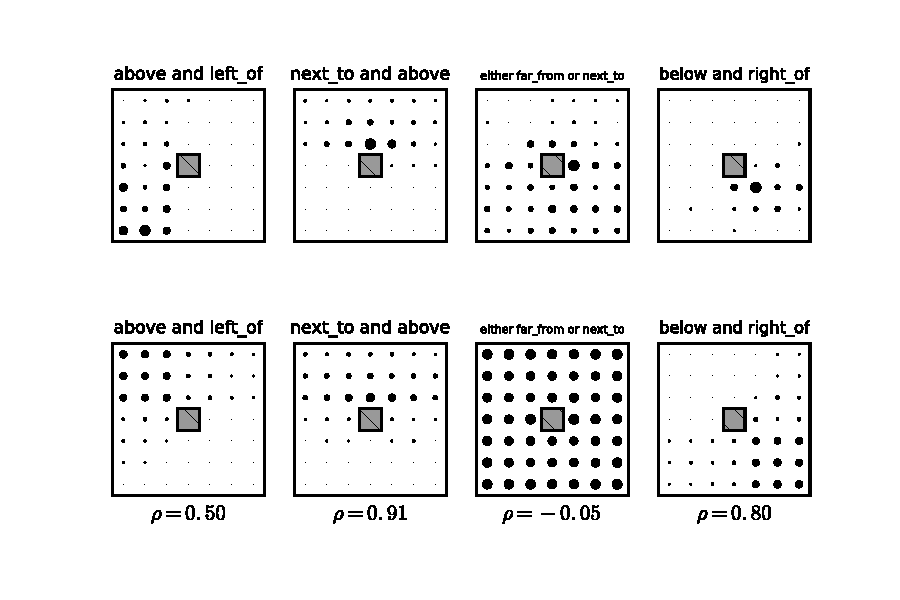
\includegraphics[width=0.8\linewidth]{studies/iwcs2017/experiment1/exp01.pdf}
\caption{\label{iwcs2017:fig:exp1:sample2} The predicted spatial templates are shown on the top and the
original spatial templates in the bottom.}
\end{figure}
The results indicate that the model can produce spatial
templates for novel compositions. However, the learning of composed phrases is
dependent on the size and the variety of training instances. Some phrases are
more difficult to train than others. For example, OR phrases correspond to
regions that are more spread out across the 48 locations which makes them more difficult to
learn, e.g. an extreme case such as ``either far from or next to''.

\subsubsection{Learning of novel single words from grounded compositions}
In this experiment we omit identical proportions of all description types, thus
also single word descriptions and negated descriptions. In this case, the predicted
novel spatial templates are learned solely based on observing these words in
combination with other words. As before, we conduct the test with different sizes
of held-out data. The results are shown in Table~\ref{iwcs2017:tab:exp1-2}. When omitting up to 4 single descriptions (\textit{right\_of}, \textit{over}, \textit{far\_from} and \textit{under}) the average
$\rho$ on grounded SINGLE-word descriptions decreases only by 0.05 (from 0.92, Table~\ref{iwcs2017:tab:exp0}). This
means that their grounding is successfully learned from grounded composed
expressions. Figure~\ref{iwcs2017:fig:exp1:above} shows a novel learned spatial
template for ``above''.

\begin{table}[tbh]
	\centering
	\small
	\begin{tabular}{lrrrr}
	\hline
	{} &   10\% &   20\% &   30\% &   40\% \\
	\hline
	AND-phrases & 0.86 &  0.8 & 0.77 & 0.81 \\
	NEG-phrases & 0.83 & 0.64 & 0.59 & 0.43 \\
	OR-phrases  & 0.73 & 0.78 & 0.68 & 0.69 \\
	SINGLE-word &  0.9 &  0.9 & 0.84 & 0.87 \\
	\hline
	\end{tabular}\vspace{0.5em}
	\caption{The average Spearman's $\rho$ %
	for different proportions of unseen examples.}\label{iwcs2017:tab:exp1-2}
\end{table}
\begin{figure}[tbh]
    \centering
    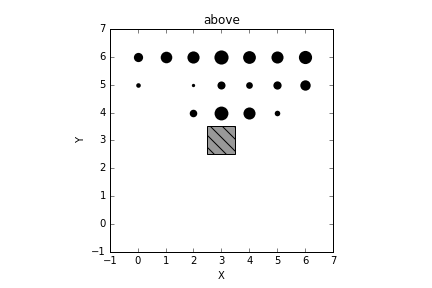
\includegraphics[width=0.4\linewidth]{studies/iwcs2017/experiment1/above_learned.png}
    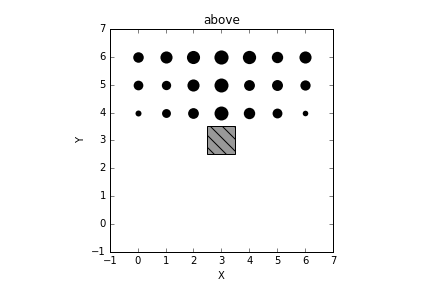
\includegraphics[width=0.4\linewidth]{studies/iwcs2017/experiment1/above_trained.png}
    \caption{\label{iwcs2017:fig:exp1:above} The predicted and the original spatial template.}
\end{figure}

\subsubsection{Qualitative observations}

A qualitative examination of the predicted spatial templates
shows that spatial templates with the lowest $\rho$ are those with no points in space
(``right\_of and left\_of'') or those with a uniform spread of points across space (``either
far\_from or next\_to'') which in our scenario includes a number of training
instances as rules from Section~\ref{iwcs2017:sec:synth} were applied to all combinations of spatial templates. We get the highest $\rho$ with compositions such as ``over and above'', possibly because the two spatial templates overlap and result in a simplified composed representation.

\subsection{Experiment 2: Adding distractor words with no spatial grounding}

In Experiment 2 we train and measure the performance of the model on grounded
descriptions which also include non-grounded distractor words, for
example: ``the ball is not left\_of the box'' or ``it is above
and right\_of the object''. The words such as ``ball'',
``object'', ``box'', ``it'' and ``is'' provide no
contribution to the grounded meaning (location). In this dataset the number of
possible composed phrases increases from 200 to 1,000. Algorithm~\ref{iwcs2017:alg:generator} in Section~\ref{iwcs2017:sec:synth} ensures that in the 1,000 possible
phrases the same number of instances is generated as before, now per each of the five permutation rules introducing distractors.
The held-out proportions of
spatial descriptions are created before Algorithm~\ref{iwcs2017:alg:generator} is applied so
permutations including these are not generated.

\subsubsection{Learning of novel grounded compositions}

Although now the training data includes longer sequences and several distractors which make these
compositions harder to learn, the results are only slightly weaker than in
Experiment 1 as shown by a comparison of Table~\ref{iwcs2017:tab:exp21} with Table~\ref{iwcs2017:tab:exp1}.

\begin{table}[htbp]
\centering
\small
\begin{tabular}{m{5.7em}c@{\hspace{0.7em}}c@{\hspace{0.7em}}c@{\hspace{0.7em}}c@{\hspace{0.7em}}c@{\hspace{0.7em}}c@{\hspace{0.7em}}c@{\hspace{0.7em}}c@{\hspace{0.7em}}}
\hline
Proportions of 90 combinations &   10\% &   20\% &   30\% &   40\% &   50\% &   60\% &   70\% &   80\% \\
\hline
AND-phrases & 0.82 &  0.79 & 0.75 & 0.78 & 0.73 & 0.69 & 0.66 & 0.45  \\
OR-phrases  & 0.78 & 0.69 & 0.67 & 0.66 & 0.59 & 0.59 & 0.44 & 0.33  \\
\hline
\end{tabular}\vspace{0.5em}
\caption{\label{iwcs2017:tab:exp21} The average
Spearman's %
$\rho$ %
with the median p-value of $<0.001$. After 80\% of held-out phrase types
the $\rho$ values are not statistically significant. }
\end{table}

\subsubsection{Learning of novel single words from grounded compositions}

The results of this task on the dataset from Experiment 2 are shown in
Table~\ref{iwcs2017:tab:exp2}. The $\rho$ are nearly identical or only slightly lower
for SINGLE-words compared to Experiment 1 (Table~\ref{iwcs2017:tab:exp1-2}). There is an
unusual drop in $\rho$ at 20\% of held-out descriptions which requires further
investigation. Overall, we can conclude that the system successfully learned
omitted single words from their grounded compositions even with distractor
words.

\begin{table}
\centering
\small
\begin{tabular}{lrrrr}
\hline
{} &   10\% &   20\% &   30\% &   40\% \\
\hline
AND-phrases & 0.82 &  0.60 & 0.71 & 0.81 \\
NEG-phrases & 0.75 & 0.66 & 0.45 & 0.30 \\
OR-phrases  & 0.76 & 0.76 & 0.71 & 0.64 \\
SINGLE-word &  0.88 &  0.43 & 0.73 & 0.84 \\
\hline
\end{tabular}\vspace{0.5em}
\caption{\label{iwcs2017:tab:exp2}The average Spearman's correlations decomposition task
Experiment 2.}
\end{table}

\begin{figure}
	\centering
	\begin{minipage}[b]{0.7\linewidth}
	    \centering
	    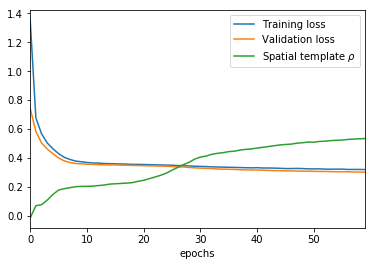
\includegraphics[width=0.75\linewidth]{studies/iwcs2017/experiment3/learning_curve.png}
	    \caption{\label{iwcs2017:fig:exp3:learning} The learning curve for Experiment 3.}
	\end{minipage}%
\end{figure}

\subsection{Experiment 3: How much grounding?}

In Experiment 3, we examine how the amount of training corresponds to the
groundedness of expressions in spatial templates. In particular, we examine the
learning curve across several epochs at which more of the same data is presented
incrementally to the learner and how well does the currently learned model
corresponds to the target spatial templates. Typically, the
performance of the learner at each epoch is estimated by a loss function, here the
cross-entropy (log-loss). We compare the loss at each epoch with the
average Spearman's $\rho$ between the predicted templates and the original
templates for 110 possible combinations of descriptions
from Experiment 1 (excluding OR-phrases). Here, we only run the experiment with 20\% omission of the
dataset. Figure~\ref{iwcs2017:fig:exp3:learning} shows how average $\rho$ corresponds to
the learning progress. The figure shows that even after the training and the validation loss are only slightly decreasing between epochs the groundedness is increasing at a higher rate. This can be explained by the fact that the network is not only predicting locations but also sequences of descriptions which adds a further complexity to learning which is reflected in the loss.


\section{Conclusion and future work}\label{iwcs2017:sec:conclusions}

We have presented a grounded language model with recurrent deep
neural networks. The objective of our task was to examine to what extent our
neural network architecture can learn a grounded language model that generated
the training data and whether a word that is grounded as a part of a phrase can
``carry over'' its grounding to another phrase not observed in the training
data. In our view this is the ultimate test that grounding is compositional. We
conduct two learning experiments. In the first experiment we learn a grounded
language model where all descriptions in a sequence are grounded. In the
subsequent sub-experiments we test the success of the grounded language models
where some word compositions are omitted from training. We show that the model is
capable of grounding novel compositions and also predicting grounding of single
words while only learning from compositions. However, the degree of success, while
on overall high, is dependent on the amount of the absent information and the
coverage of the training instances. In the second experiment, we add words to our
grounded language model that have no grounding and test whether the system is
able to learn different grounding sensitivities of different words. We show that
our language model is capable of recognising the contribution of each
constituent to the meaning of the entire grounded composition. Finally, in the
third experiment we examine grounding related to the log-loss success rate of
learning. Overall, we conclude that our deep neural architecture successfully
learns grounded spatial descriptions in a way that the learned functions are similar to the ones that generated the data.
This is a useful result which points towards the fact that language is
compositional both at the level of word sequences and the portions of scenes
that they refer to, thus confirming the result in \cite{Dobnik:2017ac}. In the future work we will focus on the effects of the
varying dataset sizes on the rate of learning and test the learning setup on
more complex perceptual representations (in terms of the expected
irregularities) such as images.


\clearpage
\bibliographystyle{acl_natbib}
\bibliography{studies/iwcs2017/references.bib}
